Para asegurar la reproducibilidad de los resultados, se detallaran a continuación la infraestructura utilizada en la ejecución del experimento, especificando tanto el hardware como el entorno software.

\subsubsection*{Hardware}
\begin{itemize}
    \item \textbf{Procesador:} Apple M2
    \item \textbf{RAM:} 16 GB (con 3.2 GB en uso durante los experimentos)
    \item \textbf{Almacenamiento:} SSD NVMe
\end{itemize}

\subsubsection*{Software}
\begin{itemize}
    \item \textbf{Sistema Operativo:} macOS 15.0.1
    \item \textbf{Compilador:} g++ (versión por defecto para macOS 16.0.0, ajustado para el soporte ARM64 en M2) y se utilizó un entorno de python con la versión 3.13
    \item \textbf{Entorno de Ejecución:} Terminal WezTerm, Shell ZSH 5.9
    \item \textbf{Entorno Gráfico:} Aqua DE con Quartz Compositor
\end{itemize}

Esta configuración garantiza que los experimentos sean replicables bajo condiciones similares. Se utilizó el comando \texttt{neofetch} para obtener los detalles de la infraestructura, que se incluyen como referencia en la Figura \ref{fig:neofetch}.

\begin{figure}[H]
    \centering
    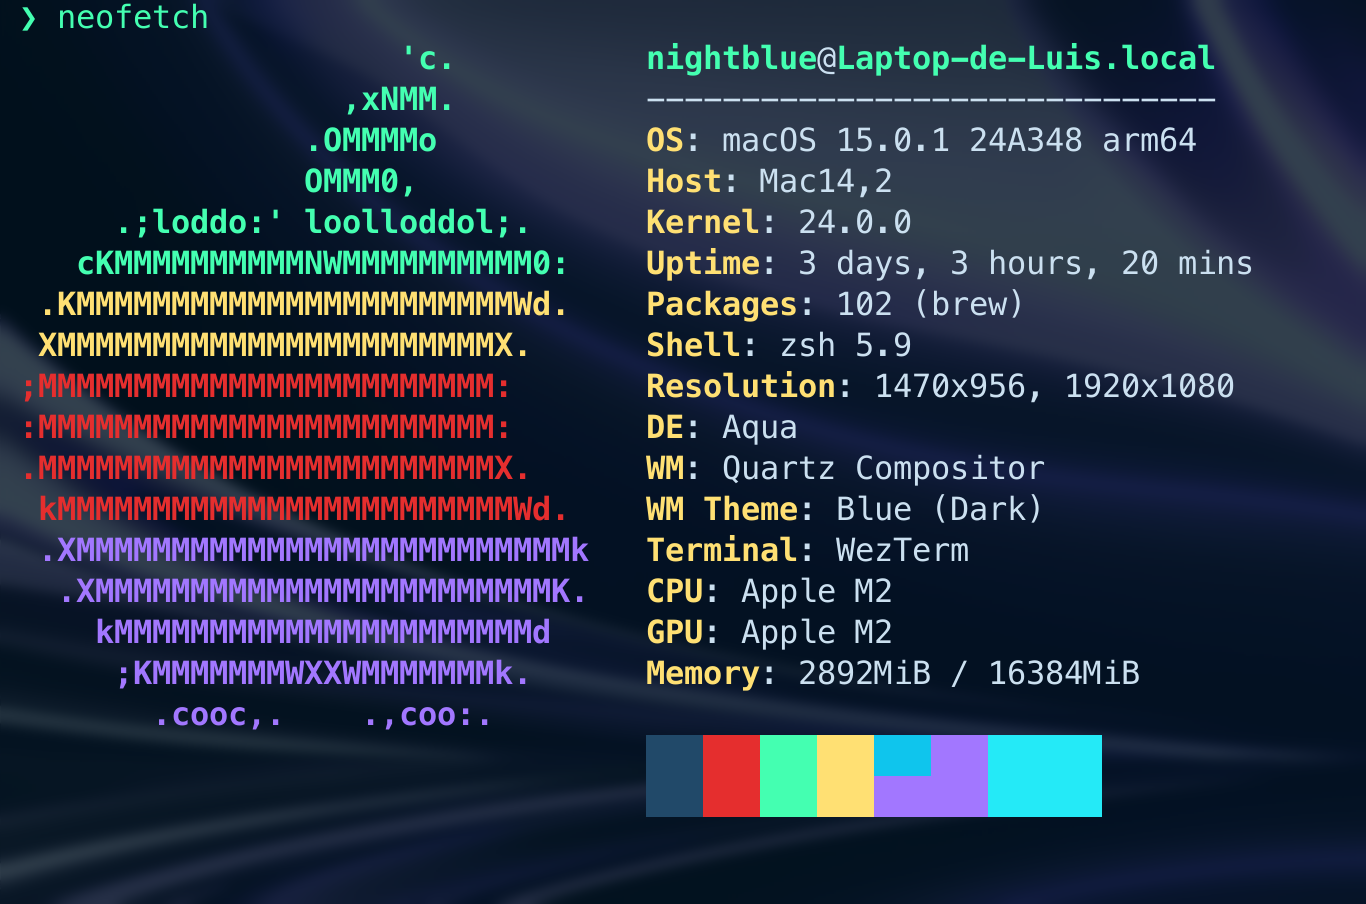
\includegraphics[width=0.7\textwidth]{images/neofetch.png}
    \caption{Detalle del sistema usando el comando \texttt{neofetch}.}
    \label{fig:neofetch}
\end{figure}

\subsection*{Condiciones de Entrada y Parámetros}

Cada experimento fue ejecutado bajo las siguientes condiciones de entrada y parámetros específicos:
\begin{itemize}
    \item \textbf{Cadenas de Entrada:} Se utilizaron cadenas de prueba de diferentes longitudes y combinaciones de caracteres para evaluar el rendimiento de los algoritmos de distancia mínima de edición (alfabeto inglés en letras minúsculas). 
    \item \textbf{Parámetros de Algoritmos:} Los costos para inserción, eliminación, sustitución y transposición fueron establecidos de acuerdo a las especificaciones de los algoritmos.
    \item \textbf{Orden de ejecución de archivos:} Primero se deben crear los archivos de costos (en caso de que no estén creados o se quieran cambiar); luego se debe ejecutar el \verb|main.cpp|, este sobreescribirá los archivos de los resultados y operaciones; por último, ejecutar el archivo Python si se quieren obtener las gráficas.
\end{itemize}

Es importante mecnionar, que esta implementación utiliza la biblioteca \texttt{sys/resource.h} de C++, la cual permite la lectura del consumo de memoria en las operaciones, pero solo está disponible en entornos Linux y Unix. En caso de utilizar un entorno diferente, será necesario eliminar esta funcionalidad en el archivo \textbf{main.cpp}. Esto implicará realizar modificaciones tales como eliminar la función de lectura de memoria del \texttt{main} y omitir la escritura de este dato en el archivo de resultados.



% Autor
% Luis Zegarra Stuardo
% 202073628-6
% Tarea 2 y 3
% Algoritmos y Complejidad 2024-2